\chapter{Methodology}

This chapter describes the adopted method for collecting relevant constraints, relating these to the common security-goals of CIAA, and later mapping them to functionality within ArchUnit. Second, this chapter presents the validation plan for expressing security constraints with ArchUnit (as is) by means of an illustration and for expressing additional constraints by means of a controlled experiment.

\section{Data collection}\label{sec:data_collection}

The relevance of the security architectural constraints included in the study was ensured by performing a review of security measures and common weaknesses and compiling the result to a list of constraints. Completeness was not the primary goal of the review, but rather to provide a set of constraints derived from previous knowledge. Presented below are the three sources used to form the final list. 

\textbf{CAWE catalog:}
The Common Architectural Weakness Enumeration catalog \cite{santos_catalog_2017} details 224 common weaknesses in security architectures. Each entry has a description of the weakness and exemplifications of how it could manifest itself in the source code, when applicable. In some entries, there are recommendations on what techniques can be used to detect the weakness, along with mitigation strategies.

\textbf{Security patterns:}
Similar to the usage of general design patterns made famous in \cite{gamma_design_1995}, security patterns provide a reusable and domain-independent solution to a known problem. More specifically, this study focused on security patterns for the design phase, as defined in \cite{yoshioka_survey_2008}. While the security pattern repository\footnote{http://sefm.cs.utsa.edu/repository/} lists over 170 security patterns, not all are provided with sufficient detail or at the appropriate level of abstraction. As a result, the report by Scandariato et al. \cite{scandariato_system_2006}  which provides a filtered list of patterns.


\textbf{Security rules:} \label{subsec:security_rules}
Architectural security rules constrain the implementation of a system while being less solution-oriented compared to security patterns. Eden and Kazman differentiate architectural security rules from those defined on a level of source code based on two criteria, locality and intension/extension \cite{eden_architecture_2003}. Architectural rules are both non-local and intensional, meaning that they affect all or several parts of the system while having \say{infinitely-many possible instances}. In \cite{franch_constraining_2019}, Jasser presents a catalog of architectural security rules. Although the entire catalog of 150 security rules is not yet available, the initial list of 22 included in the paper was used in our study.

\section{Filtering}\label{sec:processing}

%Elaborate. Perhaps explaining how the sources were analyzed. Did you analyse one right after the other, were there iterations, did you meet after each iteration to discuss your findings and synchronize individually derived subset, or did you work together? How many constraints were taken from individual sources, which of those were grouped? What is the proportion of CIAA coverage in the final list (Show CIAA in table 4.2 and show #ID linking the chosen ones from 4.1)? What was the rational for grouping? Perhaps explicitly enumerating  the "rules" you followed for inclusion would be nice (if there are more than two :) ...), e.g.:
%1) only security related architectural constraints were considered
%2) only constraints that can be enforced statically (FYI: prepare for the question, what is an example of a constraint that can not be statically enforced?),
%3) ...
Starting from each of the three sources of architectural constraints described in Section~\ref{sec:data_collection}, the first step of the process, shown in Figure~\ref{fig:mapping_process}, was to select the entries that could be formulated as enforcable constraint in the context of our project. The criteria for inclusion were the following: 

\begin{enumerate}
    \item The entry must be related to the architectural design of a system, i.e., non-local and intensional (as described in section \ref{subsec:security_rules}. \label{criterion_1}
    \item It must be possible to enforce the entry through static analysis. An example on a non enforceable constraint is "No two instances of a microservice are deployed on the same machine", as the number of machines deployed is a dynamic property. \label{criterion_2}
    \item Although somewhat included in the first criterion as it is a local issue, an entry must not relate to the correctness or best practice of the implementation of an algorithm. Examples include the practice of using session tokens with time-limited validity. \label{criterion_3}
    \item The entry must only relate to the system under design, thus ignoring the correctness and security of any external dependencies. An example can be found in SonarQube where the usage of a version of a library with known vulnerabilities is reported as a weakness. \label{criterion_4}
    \item The entry must not be dependent on externally defined data. A common example is that of user permissions where the mapping between a regulated functions and a users rights is performed using an access control list. \label{criterion_5}
    \item Additionally, we deemed measures defined as the absence of certain functionality as less valuable due to the increased difficulty of enforcement \cite{haley_security_2008}.
\end{enumerate}

\begin{figure}
    \centering
    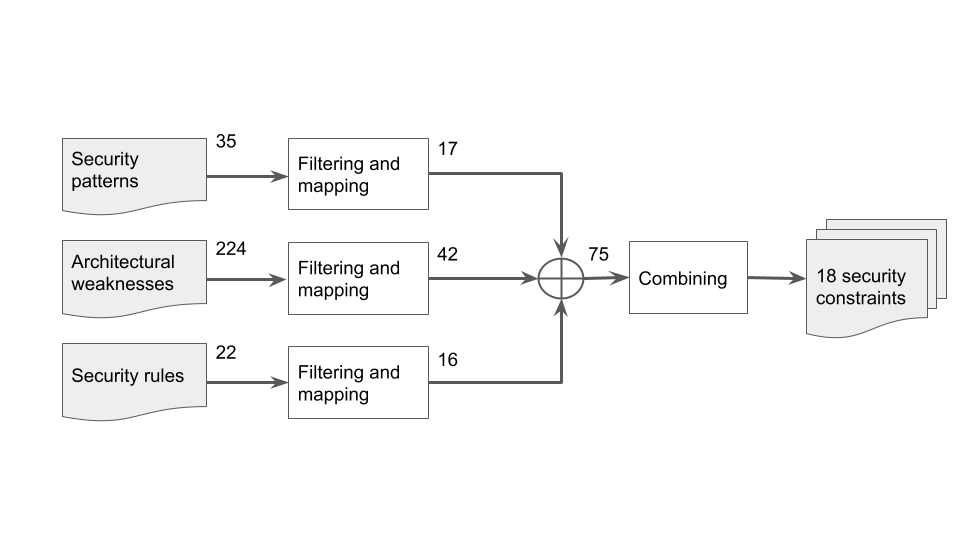
\includegraphics[width=\textwidth]{figure/Half-time presentation.png}
    \caption{Overview of the process of mapping the three sources to constraints}
    \label{fig:mapping_process}
\end{figure}

Previous research on design notations of secure systems have shown a skew towards confidentiality and integrity while having little or no support for availability and accountability. We considered it necessary for the final list of constraints to include all of the security goals. As a consequence, once we had selected the applicable entries, we categorized them according to the security goals of CIAA, ensuring that the final list of constraints covered all security goals. 

The last part of compiling a list of security architectural constraints involved combining the selected entries to remove duplicates and group similar concepts. Duplication involved both a single source having several entries, such as CAWE having input validation weakness for multiple tools and technologies (e.g., SQL, LDAP) and different sources having entries for the same concept, such as the security pattern input guard and the previously mentioned input validation weaknesses. Grouping similar concepts also allowed for the constraints to be more general, thus making them applicable for a broader set of systems. 

\section{Validation}

The validation of our results will be performed in two ways, depending on whether or not a constraint required any modification of ArchUnit or additional information in the source-code. The latter category carries a higher degree of scientific value thus motivating a more thorough validation procedure. In the sections below, both types of procedures will be described. 

\subsection{Solution Proposal}

As described in Section~\ref{archunit-back-section}, ArchUnit already provides functionality to perform conformance testing of architectural constraints. However, it is unclear whether the framework supports the enforcement of security architectural constraints. The mapping of security architectural constraints to that of rules in ArchUnit allows us to perform a \textit{proposal of solution} as described in \cite{wieringa_requirements_2006}. This type of validation is intended to propose a novel or significantly improved technique without rigorous validation. Instead, a proof of concept or small example is used to facilitate later validation. 

\subsection{Controlled Experiment} \label{sec-controlled-experiment}
In contrast to constraints which may be implemented through already existing functionality, those requiring extension to either the API or additional information within the source-code are not guaranteed to reliably detect violations of the intended architecture. Therefore, validation is performed using a laboratory experiment \cite{stol_abc_2018} in order to increase the precision of the measurement. 

Integration with already existing testing frameworks is a prominent advantage of ArchUnit. As testing is generally performed overtime to ensure that a system does not degrade, the focus of the experiment is to determine whether ArchUnit can detect changes to security architectural constraints between two versions. 

\subsubsection{Performance metrics}
The imbalance between the designer, who needs to ensure that every single aspect of a system is secure, and the attacker, who needs to succeed only once, influences the metrics chosen to represent how well the extension to ArchUnit performs. Precision and recall were the metrics of choice, with the greater importance placed on the latter. 

\subsubsection{Projects used in evaluation}
Systems to be included in the validation needed to fulfill two mandatory criteria. First and foremost was the fact that they need open source and written in Java as the static analysis of ArchUnit relies on the source-code. Secondly, there needed to be at minimum two different snapshots in order to fulfill the goal of comparing subsequent changes to a system.  

In addition to the mandatory criteria, other aspects were also considered to reduce bias in the validation process. Systems which had already been analyzed in previous literature \cite{peldszus_secure_2019, abi-antoun_static_2009} would provide an existing architecture and its security analysis, which we leverage as ground truth in our experiment. Additionally, systems which have a well documented architecture and security requirements and were within a reasonable size can further help mitigate potential internal validity threats. 